%*****************************************************************
%*************************** Section 5 ***************************
%********************* Lenkung des Fahrzeugs *********************
%*****************************************************************


\pagestyle{fancy}
\rhead{\thepage} \chead{} \lhead{\ref{Sec5}. \nameref{Sec5}}
\cfoot{}

\section{Lenkung des Fahrzeugs}\label{Sec5}

Wie in Kapitel \ref{Sec2Sub1} beschrieben, wird das Lenkgestänge des Fahrzeugs von einem Servomotor angetrieben, der im Folgenden näher erklärt wird. Auch auf die Montage der Antriebskomponenten und die Programmierung des Lenkungsbausteins wird in diesem Kapitel näher eingegangen.

\subsection{Servoantrieb}\label{Sec5Sub1}

Zur Lenkung des Fahrzeugs wird ein Servomotor (siehe Abbildung \ref{fig:ServoMotor}) verwendet, der mit den Achsen über ein Lenkgestänge verbunden ist. Ein Servo besteht aus einem Motor, dessen Welle mit einem Potentiometer verbunden ist. Die interne Elektronik regelt automatisch die Istwert-Vorgabe des Potentiometers auf den an der Signalleitung anliegenden Sollwert aus. Dadurch können Lenkwinkelpositionen genau angefahren werden. Die Sollwert-Vorgabe erfolgt wie die Drehzahlvorgabe bei den \acp{BLDCMot} mit einem 50Hz \ac{PWM}-Signal und einem Tastgrad von 5\% bis 10\%, wobei dieser proportional zum Lenkwinkel ist. Bei einem Tastgrad von 7,5\% befindet sich die Lenkung in der Mittelstellung. Kleinere Werte bewirken einen Lenkeinschlag nach links und größere Werte einen Einschlag nach rechts. Der \ac{PWM}-Signalleitung und der dazugehörigen Masseleitung schließt sich noch eine Versorgungsleitung an (5V-Versorgung).

\begin{figure}[H] %H für Positionierung hier
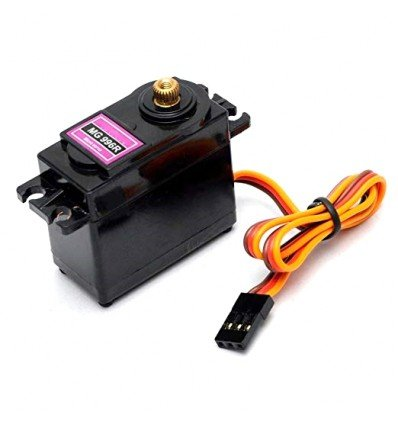
\includegraphics[width=.50\textwidth]{sec5/images/Servo.jpg} 
\centering
\captionsetup{width=.95\textwidth}
\caption[Servomotor mit Anschlussleitungen~\cite{DIYE}]{Servomotor mit Anschlussleitungen; Versorgungsspannung rote Leitung, \ac{PWM}-Signal orangene Leitung und Masseleitung in braun~\cite{DIYE}}\centering
\label{fig:ServoMotor}
\end{figure}

\newpage
\subsection{Montage der Lenkungskomponenten}\label{Sec5Sub2}

Die Komponenten der Lenkung, welche über einen Servomotor und ein mit den Reifen verbundenes Lenkgestänge realisiert ist, sind wie die Antriebskomponenten auf der unteren Fahrzeugebene montiert. Der Servomotor ist mit vier Schrauben an einem losen Teil des Chassis befestigt, welches über zwei Schrauben durch Langlöcher von oben am Fahrzeug montiert ist. Über die Langlöcher kann der Servomotor so platziert werden, dass die Vorderreifen parallel zueinander stehen. An der Welle des Servomotors ist dann das Lenkgestänge befestigt, welches mit den Reifen verbunden ist.\vspace{11pt}

In Abbildung \ref{fig:MontageLenkungskomponenten} sind die montierten Komponenten der Fahrzeuglenkung abgebildet. Die Befestigung des Servomotors ist in violett hervorgehoben, die Befestigung des losen Chassis-Teils in rot, die Lenkgestänge in blau und die Federung in orange.

\begin{figure}[H] %H für Positionierung hier
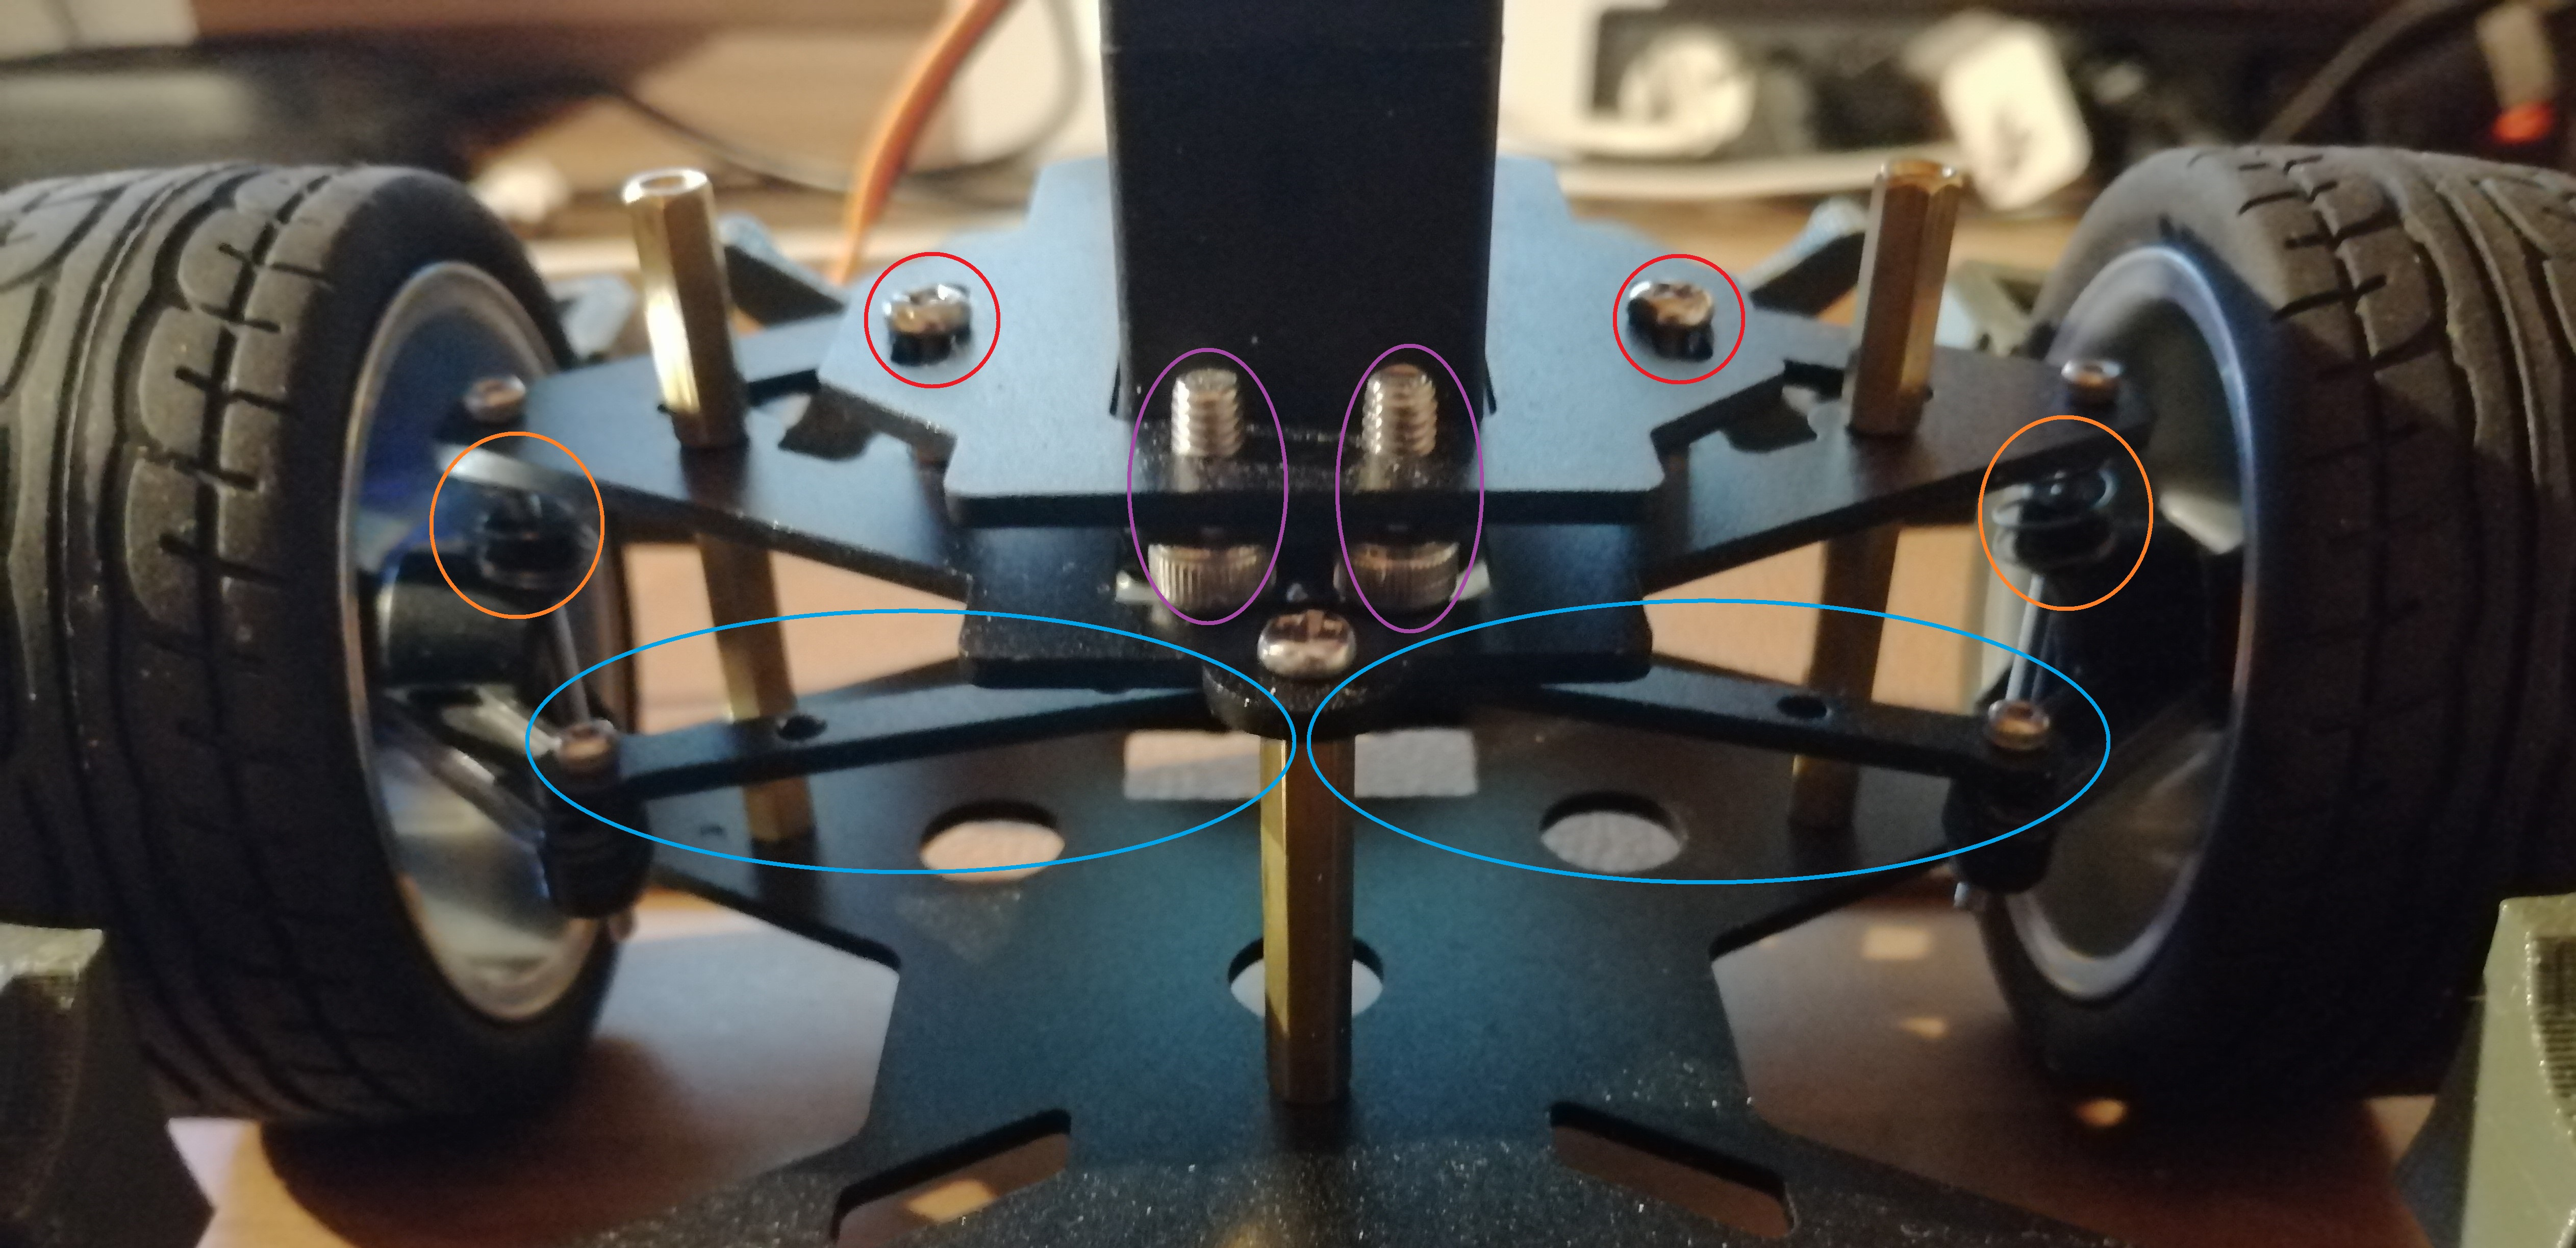
\includegraphics[width=.90\textwidth]{sec5/images/MontageLenkungskomponenten} 
\centering
\captionsetup{width=.95\textwidth}
\caption[Montage der Lenkungskomponenten]{Montage des Servo-Motors, des Lenkgestänges und der Vorderreifen; Befestigung des Servo-Motors in violett, Befestigungsschrauben des losen Chassis-Teils in rot, Lenkgestänge in blau und Federung in orange}\centering
\label{fig:MontageLenkungskomponenten}
\end{figure}

\newpage
\subsection{Programmierung des Lenkungsbausteins}\label{Sec5Sub3}

Der Lenkungsbaustein der Software ist wie der Antriebsbaustein in zwei Dateien unterteilt, die Dateien \glqq{}servo.c\grqq{} und  \glqq{}servo.h\grqq{}. Die Datei \glqq{}servo.h\grqq{} enthält alle relevanten Bibliotheken und Prototypen für die Datei \glqq{}servo.c\grqq{}. Außer der Einbindung der Bibliotheken und der Prototypen der Funktionen aus der Datei \glqq{}servo.c\grqq{} sind hier auch die Parameter für die Initialisierung des Timers für das \ac{PWM}-Signal hinterlegt (Abbildung \ref{fig:ServoH}). 

\begin{figure}[H] %H für Positionierung hier
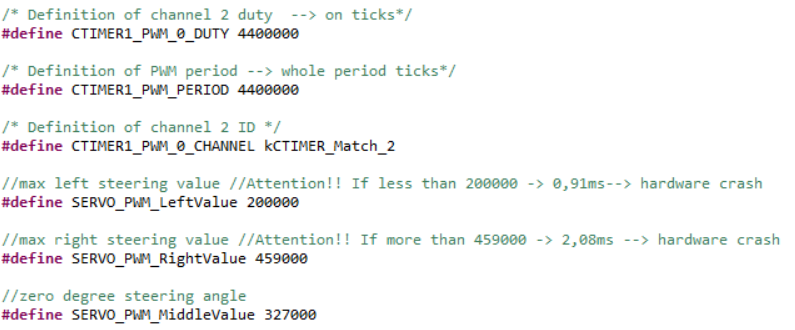
\includegraphics[width=.90\textwidth]{sec5/images/ServoH} 
\centering
\captionsetup{width=.95\textwidth}
\caption[Relevante Zeilen der Datei \glqq{}servo.h\grqq{}]{Relevante Zeilen der Datei \glqq{}servo.h\grqq{} mit den Parametern für die Initialisierung des \ac{PWM}-Timers}\centering
\label{fig:ServoH}
\end{figure}

Wie schon beim Antrieb, wird für die \ac{PWM}-Periodendauer bei der Initialisierung ein Wert von 4.400.000 Takten festgesetzt, woraus mit einer \ac{CPU}-Taktfrequenz von 220MHz (220.000.000 Takte pro Sekunde) eine Periodendauer von 20ms resultiert. Die Pulsbreite wird während des Programmablaufs regelmäßig überschrieben, weshalb für die Initialisierung ein Wert von 0 gewählt werden kann. So bewegt sich der Servomotor bei der Initialisierung nicht und es kommt dabei nicht zum Crash.\vspace{11pt}

Der Wert für den linken maximalen Lenkeinschlag (ca. 200.000) entspricht einer \ac{PWM}-Pulsbreite von 0,91ms und der des maximalen rechten Lenkeinschlags (ca. 459.000) einer Breite von 2,08ms. Auch wenn der Servomotor einen Wert zwischen 1ms und 2ms erwartet, kann mit den eben genannten Einstellungen noch ein wenig mehr Lenkeinschlag gewonnen werden. Mit dem Wert der Mittelstellung (ca. 327.000), welcher durch Probieren angenähert wurde, beläuft sich die Pulsbreite auf 1,486ms. Alle drei Extremwerte (\glqq{}servoMiddleValue\grqq{}, \glqq{}servoLeftValue\grqq{}, \glqq{}servoRightValue\grqq{}) sind Parameter, deren Werte aus dem \ac{EEPROM} kommen und welche über das Bedienungsboard eingestellt werden können (siehe Abbildung \ref{fig:ServoC0}).

\begin{figure}[H] %H für Positionierung hier
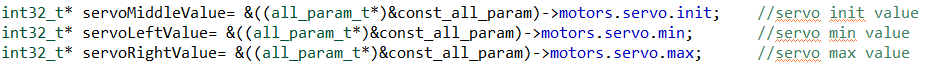
\includegraphics[width=.95\textwidth]{sec5/images/ServoC0} 
\centering
\captionsetup{width=.95\textwidth}
\caption[Extremwerte der Lenkwinkel als Parameter aus dem \ac{EEPROM}]{Extremwerte der Lenkwinkel als Parameter aus dem \ac{EEPROM}, deren Werte über das Bedienungsboard individuell einstellbar sind; Teil der Datei \glqq{}servo.c\grqq{}}\centering
\label{fig:ServoC0}
\end{figure}

Auch der \ac{PWM}-Timer benötigt bei der Initialisierung einige Parameter, deren Werte in der Datei \glqq{}servo.h\grqq{} festgelegt sind (\ac{PWM}-Periodendauer, \ac{PWM}-Pulsdauer, Channel). Der Channel wird auf das Timer Match Register 2 festgelegt (\glqq{}kCTIMER\_Match\_2\grqq{}), was bei dem verwendeten Controller dem Pin P3.2 entspricht. Der Pin P3.2 wird auf der Controllerplatine über den Pin 11 der Buchsenleiste J13 nach außen geführt.

\begin{figure}[H] %H für Positionierung hier
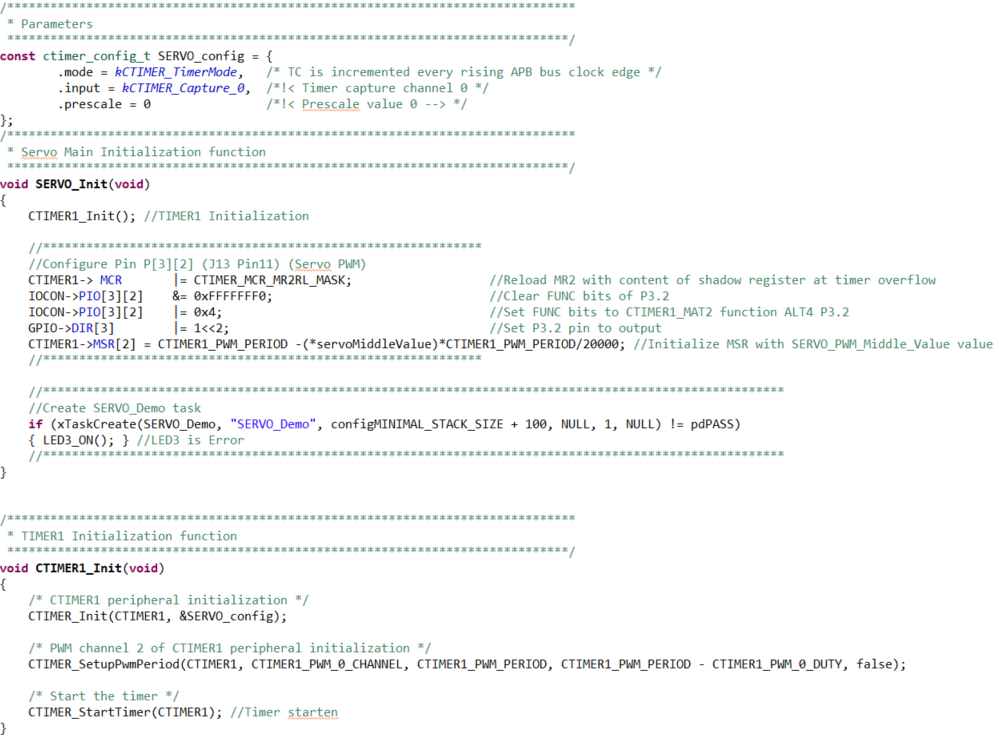
\includegraphics[width=.95\textwidth]{sec5/images/ServoC1} 
\centering
\captionsetup{width=.95\textwidth}
\caption[Funktionen SERVO\_Init, CTIMER1\_Init und SERVO\_Demo der Datei \glqq{}drive.c\grqq{}]{Funktionen SERVO\_Init und CTIMER1\_Init und Demonstrations-Task SERVO\_Demo der Datei \glqq{}drive.c\grqq{}}\centering
\label{fig:ServoC1}
\end{figure}

Die Datei \glqq{}servo.c\grqq{} enthält die Funktionen zur Initialisierung der für die Verwendung des Servos notwendigen Controller-Peripherie. In der Funktion SERVO\_Init wird zuerst die Funktion CTIMER1\_Init aufgerufen, welche den Timer mit den in der Datei \glqq{}servo.h\grqq{} festgelegten Parametern als \ac{PWM}-Timer mit einer Periodendauer von 20ms und einer Pulslänge von 0ms initialisiert. Im Anschluss daran wird festgelegt, dass bei einem Timer-Überlauf die neuen Daten für die Pulslänge aus dem Shadow-Register geladen werden sollen. Zum Ändern des Lenkwinkels muss deshalb lediglich ein neuer Wert in das Shadow-Register geschrieben werden. Hier muss allerdings aufgepasst werden, da das Register nicht die Pulsbreite (On-Time) sondern die Off-Time erwartet. Deshalb muss der Wert, der eingetragen wird, der Periodendauer abzüglich der Pulsdauer entsprechen. Zusätzlich wird in der Funktion SERVO\_Init auch der Pin 3.2 für die Verwendung als \ac{PWM}-Ausgang des Timers C konfiguriert (siehe Abbildung \ref{fig:ServoC1}).\vspace{11pt}

Am Ende wird der Wert für die Mittelstellung des Servos in das Shadow-Register geschrieben und ein Task für die Demonstration der Lenkung gestartet (SERVO\_Demo), welcher nach einmaligem Linkslenken, Rechtslenken und nach der Rückkehr in die Mittelstellung ausgesetzt wird. Der Task \glqq{}SERVO\_Demo\grqq{} ist in Abbildung \ref{fig:ServoC2} einsehbar.

\begin{figure}[H] %H für Positionierung hier
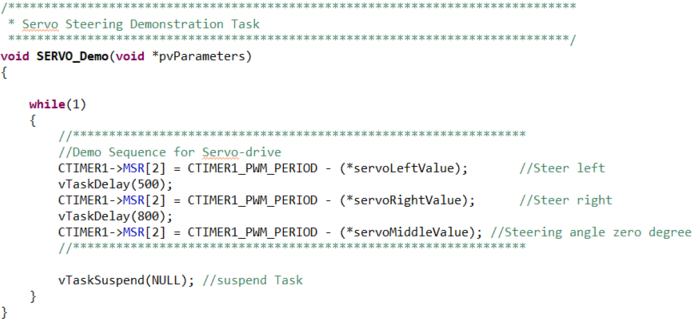
\includegraphics[width=.85\textwidth]{sec5/images/ServoC2} 
\centering
\captionsetup{width=.95\textwidth}
\caption[SERVO\_Demo Task der Datei \glqq{}drive.c\grqq{}]{SERVO\_Demo Task der Datei \glqq{}drive.c\grqq{}}\centering
\label{fig:ServoC2}
\end{figure}

\newpage